%
% Time domain
%
Before considering the introduction of temporal modelling to information systems, it is necessary to define and explain some main concepts concerning temporal modelling and their corresponding terminology, to situate these and to discuss some properties and issues related to these concepts. In this section, several basic concepts and corresponding terminology will be defined, explained and situated. Most of these concepts are widely used in the community of temporal databases and their definitions have been agreed upon in the context of~\cite{Dyreson1994}. For these concepts, in the entire chapter, the contents of~\cite{Dyreson1994} are followed (and often cited).

In subsection \ref{subsec:basic-concepts}, some basic concepts of time modelling are presented and explained.

%In order to define and to work with time it is necessary to study and understand the underlying domain. Moreover, the definition of a temporal domain is the basis for almost any temporal system. In the following subsection \ref{subsec:basic-concepts} we will introduce several concepts that are widely used in the community of temporal databases. Most of the concepts explained here have been introduced in the \emph{'Consensus Glossary of Temporal Database Concepts'}~\cite{Dyreson1994}.



\subsection{Basic concepts and properties}
\label{subsec:basic-concepts}
In information systems, time itself is usually percieved as a linear or cyclic concept. Therefore, a time domains modelling time is usually represented by a set with an imposed partial order. In general, two main types of time models can be discerned: a \emph{linear} model and a \emph{cyclic} model. In the linear model, a total order is imposed on the set and the progress of time is seen as a linear matter, while cyclic models are mainly used in the modelling of recurrent processes. It should be noted that the majority of proposals use linear time models.

Data models used by information systems (and in specific, temporal database systems) may represent these underlying time domains using \emph{chronons}. However, to explain what chronons are, an explanation of some other temporal concepts is necessary.

\begin{svgraybox}
\vspace{-10pt}
\begin{definition}\textbf{Instant}\\
An \emph{\textbf{instant}} is a time point on an underlying time axis.
\end{definition}
\vspace{-10pt}
\end{svgraybox}

Thus, an instant is basically an instantanious time point in a time model.

Orthogonal to the classification of underlying time models as linear or cyclic, they can be classified as \emph{discrete}, \emph{dense} or \emph{continuous} models. In a discrete model, the notion exists that every instant has a unique successor and the set of instants is seen as a discrete one. Here, intuitively, the set of instants can be seen as isomorphic to the set of natural numbers $\Nat$. In a dense model, the notion exists that between any two instants always lies another, while the set of instants can still be seen as a discrete one. Here, intuitively, the set of instants can be seen as isomporphic to the set of rational numbers $\Q$ or the set of real numbers $\R$. In a continuous model, the notion also exists that between any two instants always lies another one, but unlike dense models, the set of instants is seen as continuous and there are no ``gaps'' between successive instants.

Some other necessary concepts are:

\begin{svgraybox}
\vspace{-10pt}
\begin{definition}\textbf{Time Interval}\\
A \emph{\textbf{time interval}} is the time between two instants.
\end{definition}

\begin{definition}\textbf{Temporal Element}\\
A \emph{\textbf{temporal element}} is a finite union of time intervals.
\end{definition}

\begin{definition}\textbf{Event}\\
An \emph{\textbf{event}} is an instantaneous fact, i.e. something occurringat an instant.
\end{definition}

\begin{definition}\textbf{Duration}\\
A \emph{\textbf{duration}} is an amount of time with known length, but no specific starting or ending instants.
\end{definition}

\begin{definition}\textbf{`Temporal' as Modifier}\\
The modifier \emph{\textbf{`temporal'}} is used to indicate that the modified concept concerns some aspect of time.
\end{definition}
\vspace{-10pt}
\end{svgraybox}

%In the linear model, time advances from the past to the future in a totally ordered fashion (a relationship of total order is imposed to the set). A cyclic model of time is used for recurrent processes. The majority of the proposals work with a linear model of time.

Data models might now represent an underlying time domain using chronons:

\begin{svgraybox}
\vspace{-10pt}
\begin{definition}\textbf{Chronon}\\
In a data model, a \emph{\textbf{chronon}} is a non-decomposable time interval of some fixed, minimal duration.
\end{definition}
\vspace{-10pt}
\end{svgraybox}

A data model may now represent a time model or time domain by a sequence of consecutive chronons. These chronons have identical durations. A data model will typically not specify the exact chronon duration, so it can be fixed later by applications implementing the data model.

The fact that chronons are actually time intervals has a particular effect on the representation of instants and time intervals. In a data model representing a time domain using chronons, an instant is of course represented as a chronon, but one single chronon may represent multiple instants. A time interval may be represented by a set of contiguous chronons, depending on the amount of time the time interval comprises.

%\begin{svgraybox}
%The basic elements in a temporal domain are the following:\\
%\begin{itemize}
%\item
%\textbf{Instant}:  Is a time point over an underlying temporal domain.\\
%\item
%\textbf{Time interval}: Is the time between two instants.\\
%\item
%\textbf{Event}: Is an instantaneous fact. Something that happens at an instant.\\
%\item
%\textbf{Chronon}: Is a non-decomposable time interval of fixed duration. It is possible for a temporal model to leave the chronon duration unspecified. The duration will be specified later in the implementation of the model.
%\end{itemize}
%\end{svgraybox}

%\begin{definition}\textbf{(set of chronons)}
%\label{def:set-chronon}
%The \textbf{\emph{set of all the chronons}} in a system is denoted by $\C$. A chronon $c$ is therefore defined as:
%\begin{equation}
%\left \lbrace c \mid c \in \C \right \rbrace
%\end{equation}
%\end{definition}

Another classification of time models concerns the use of points or intervals to model time. The equivalence between interval-based and point-based time models is demonstrated in \cite{Böhlen_point-versus}.

%Attending to the density in the set $\C$ of the chronons, a model can be classified into the following three types:

%\begin{itemize}
%\item
%\textbf{Discrete model} ($\C \subset \Nat$):  The discrete model of time is isomorphic in relation to the natural numbers. %According to this model, each natural number corresponds to a \emph{chronon}.
%\item
%\textbf{Dense model} ($\C \subset \Q$ or $\C \subset \R$): This model is isomorphic in relation to the rational or the real %numbers. It represents one instant of time in the gap between another two instants. 
%\item
%\textbf{Continuous model} ($\C \subset \R$): This is an extension of the dense model with no gaps. It is isomorphic in relation to the real numbers. 
%\end{itemize}

\textcolor{red}{CHECK}
Restrictions on time range may be performed on the base of the following two concepts:
\begin{itemize}
\item
\textbf{Time boundedness}: Time can be bounded orthogonally in the past and in the future.
\item
\textbf{Time distance}: As a metric, time has a distance function which presents four properties:
\begin{enumerate}
\item
Distance is non-negative.
\item
The distance between two different elements is not equal to zero.
\item
The distance from $\alpha$ to $\beta$ is the same as that between $\beta$ and $\alpha$.
\item
Triangle inequality: The distance from $\alpha$ to $\gamma$ is equal or greater than the distance from $\alpha$ to $\beta$ plus the distance from $\beta$ to $\gamma$.
\end{enumerate}
\end{itemize}
\textcolor{red}{END CHECK}

\textcolor{red}{MOVE TO TEMPORAL DATABASE PART}
On the other hand, time may be \textbf{relative} or \textbf{absolute} (in other words, \textbf{anchored} or \textbf{unanchored}). Sometimes, what one considers \emph{absolute time} is not as definite as one would hope since our concept of absolute time is based on another time reference (for example, January 1st of year one). Relative time has a direction, differently from distance. It is also possible to use negative references so as to represent relative time (e.g. -3 days = three days ago).
\textcolor{red}{END MOVE}

Subsection \ref{subsec:granularity} gives a short survey on the concept of temporal granularities.

%%% granularity
\subsection{Granularities}\label{subsec:granularity}
An important issue in time modelling concerns the concept of \emph{temporal granularities}. A formal definition for this concept is given in~\cite{Lin97}:

\begin{svgraybox}
\vspace{-10pt}
\begin{definition}\textbf{Granularity}\\
A \emph{\textbf{granularity}} is an ordered set of non-overlapping and continuous temporal elements called \emph{granules}.
\end{definition}

\begin{definition}\textbf{Granule}\\
A \textbf{\emph{granule}} is the basic time unit in a granularity.
\end{definition}
\vspace{-10pt}
\end{svgraybox}

A temporal granularity is in fact a partitioning of the time line (time model) used by a system, usually dependent on the application. For example, the age of an adult human being is usually expressed in years: one will use sentences like `Laura is 21 years old' instead of sentences like `Laura is 21 years, 3 months and 4 days old'. In this example any duration shorter than a year needs no representation and thus the used granularity allows no specification for durations shorter than a year. The granules are years.

As a granularity $G$ is an ordered set, each granule may be represented by an integer. In this representation, to keep track of the granularity a granule is an element of, the corresponding granularity is added in subscript:

\begin{equation}
G = \left\{i_{G}\ |\ i \in \Z \right\}
\end{equation}

%Next to the inherent difficulties of time, an issue is \textbf{temporal granularity}. A temporal granularity is a partitioning of the time line used by a system, usually dependent on the application. For example, the age of an adult human being is usually expressed in years: one will use sentences like \emph{`Laura is 21 years old'} instead of \emph{`Laura is 21 years, 3 months and 4 days old'}. In this example any time period shorter than a year needs no representation and thus the used granularity allows no specification for time periods shorter than a year.
%The formal definition for granularity is given in ~\cite{Lin97}:


%\begin{definition}
%\label{def:granularity}\textbf{(granularity)}
%A \textbf{\emph{granularity}} $\alpha$ is an ordered set of non-overlapping and continuous time elements called granules. \\
%\end{definition}

%As granularity $\alpha$ it is an ordered set, each \emph{granule} may be indexed by an integer number:\\
%\begin{equation}
%\alpha = \left \lbrace \ldots, 0_\alpha, 1_\alpha, \ldots \right \rbrace
%\end{equation}

In a system, the granularity with the shortest granules is the \emph{chronons granularity}, which is denoted as $\bot$. It is the granularity of which the granules are chronons. It is now possible to define a function $f$, called a \emph{mapping function}, that maps a given granule $i_G$, $i \in \Z$, from a given granularity $G$ to a set of corresponding chronons. The function definition should look like this:
\vspace{-10pt}

\begin{align}
f & : G \rightarrow \Pow(\bot)\nonumber\\
  & : i_{G} \rightarrow \lbrace c_\bot\ |\ (c_\bot\text{ is contained in }i_{G}) \wedge (c_\bot \in \bot)\rbrace\nonumber
\end{align}

For a given granularity $G$ and a given mapping function $f$ from $G$ to $\bot$, it is required that the following properties hold:

\begin{itemize}
\item
$G$ \emph{is an ordered set}: for a given $i_{G} \in G$ holds: if $c_\bot \in f(i_G)$ and $c^{'}_\bot \in f(j_G)$, then $c_\bot < c^{'}_\bot$ implies that $i_G < j_G$. This is illustrated in figure \ref{fig:granularity-prop1}.
\begin{figure}
\centering
%%Created by jPicEdt 1.4.1_03: mixed JPIC-XML/LaTeX format
%%Mon Jan 30 18:36:37 CET 2012
%%Begin JPIC-XML
%<?xml version="1.0" standalone="yes"?>
%<jpic x-min="-5" x-max="50" y-min="-2" y-max="22" auto-bounding="true">
%<multicurve fill-style= "none"
%	 points= "(0,0);(0,0);(50,0);(50,0)"
%	 />
%<multicurve fill-style= "none"
%	 points= "(0,20);(0,20);(50,20);(50,20)"
%	 />
%<multicurve fill-style= "none"
%	 points= "(2,0);(2,0);(10,20);(10,20)"
%	 />
%<multicurve fill-style= "none"
%	 points= "(10,20);(10,20);(16,0);(16,0)"
%	 />
%<multicurve fill-style= "none"
%	 points= "(24,0);(24,0);(32,20);(32,20)"
%	 />
%<multicurve fill-style= "none"
%	 points= "(32,20);(32,20);(38,0);(38,0)"
%	 />
%<text text-vert-align= "center-v"
%	 anchor-point= "(10,22)"
%	 fill-style= "none"
%	 text-frame= "noframe"
%	 text-hor-align= "center-h"
%	 >
%$i_G$
%</text>
%<text text-vert-align= "center-v"
%	 anchor-point= "(32,22)"
%	 fill-style= "none"
%	 text-frame= "noframe"
%	 text-hor-align= "center-h"
%	 >
%$j_G$
%</text>
%<text text-vert-align= "center-v"
%	 anchor-point= "(8,-2)"
%	 fill-style= "none"
%	 text-frame= "noframe"
%	 text-hor-align= "center-h"
%	 >
%$c_\bot$
%</text>
%<text text-vert-align= "center-v"
%	 anchor-point= "(34,-2)"
%	 fill-style= "none"
%	 text-frame= "noframe"
%	 text-hor-align= "center-h"
%	 >
%$c^{'}_\bot$
%</text>
%<text text-vert-align= "center-v"
%	 anchor-point= "(0,10)"
%	 fill-style= "none"
%	 text-frame= "noframe"
%	 text-hor-align= "center-h"
%	 >
%$f(i_G)$
%</text>
%<text text-vert-align= "center-v"
%	 anchor-point= "(42,10)"
%	 fill-style= "none"
%	 text-frame= "noframe"
%	 text-hor-align= "center-h"
%	 >
%$f(j_G)$
%</text>
%<text text-vert-align= "center-v"
%	 anchor-point= "(-5,0)"
%	 fill-style= "none"
%	 text-frame= "noframe"
%	 text-hor-align= "center-h"
%	 >
%$\C$
%</text>
%<text text-vert-align= "center-v"
%	 anchor-point= "(-5,20)"
%	 fill-style= "none"
%	 text-frame= "noframe"
%	 text-hor-align= "center-h"
%	 >
%$G$
%</text>
%</jpic>
%%End JPIC-XML
%LaTeX-picture environment using emulated lines and arcs
%You can rescale the whole picture (to 80% for instance) by using the command \def\JPicScale{0.8}
\ifx\JPicScale\undefined\def\JPicScale{1}\fi
\unitlength \JPicScale mm
\begin{picture}(50,22)(0,0)
\linethickness{0.3mm}
\put(0,0){\line(1,0){50}}
\linethickness{0.3mm}
\put(0,20){\line(1,0){50}}
\linethickness{0.3mm}
\multiput(2,0)(0.12,0.3){67}{\line(0,1){0.3}}
\linethickness{0.3mm}
\multiput(10,20)(0.12,-0.4){50}{\line(0,-1){0.4}}
\linethickness{0.3mm}
\multiput(24,0)(0.12,0.3){67}{\line(0,1){0.3}}
\linethickness{0.3mm}
\multiput(32,20)(0.12,-0.4){50}{\line(0,-1){0.4}}
\put(10,22){\makebox(0,0)[cc]{$i_G$}}

\put(32,22){\makebox(0,0)[cc]{$j_G$}}

\put(8,-2){\makebox(0,0)[cc]{$c_\bot$}}

\put(34,-2){\makebox(0,0)[cc]{$c^{'}_\bot$}}

\put(0,10){\makebox(0,0)[cc]{$f(i_G)$}}

\put(42,10){\makebox(0,0)[cc]{$f(j_G)$}}

\put(-5,0){\makebox(0,0)[cc]{$\C$}}

\put(-5,20){\makebox(0,0)[cc]{$G$}}

\end{picture}

\caption{$G$ is an ordered set}
\label{fig:granularity-prop1}
\end{figure}

\item
$G$ \emph{is a set of continuous granules}: for a given $i_{G} \in G$ and given chronons $c_\bot$, $c^{'}_\bot$ and $c^{''}_\bot$ holds: if $c_\bot < c^{'}_\bot < c^{''}_\bot$, then $c_\bot \in f(i_G)$ and $c^{''}_\bot \in f(i_G)$ implies that $c^{'}_\bot \in f(i_G)$. This is illustrated in figure \ref{fig:granularity-prop2}.
\begin{figure}
\centering
%%Created by jPicEdt 1.4.1_03: mixed JPIC-XML/LaTeX format
%%Tue Jan 17 10:05:05 CET 2012
%%Begin JPIC-XML
%<?xml version="1.0" standalone="yes"?>
%<jpic x-min="-4" x-max="50" y-min="-2" y-max="20" auto-bounding="true">
%<multicurve fill-style= "none"
%	 points= "(0,0);(0,0);(50,0);(50,0)"
%	 />
%<multicurve fill-style= "none"
%	 points= "(0,20);(0,20);(50,20);(50,20)"
%	 />
%<text text-vert-align= "center-v"
%	 anchor-point= "(-4,20)"
%	 fill-style= "none"
%	 text-frame= "noframe"
%	 text-hor-align= "center-h"
%	 >
%$\alpha$
%</text>
%<text text-vert-align= "center-v"
%	 anchor-point= "(-4,0)"
%	 fill-style= "none"
%	 text-frame= "noframe"
%	 text-hor-align= "center-h"
%	 >
%$\C$
%</text>
%<multicurve fill-style= "none"
%	 points= "(14,0);(14,0);(22,20);(22,20)"
%	 />
%<multicurve fill-style= "none"
%	 points= "(22,20);(22,20);(28,0);(28,0)"
%	 />
%<text text-vert-align= "center-v"
%	 anchor-point= "(10,10)"
%	 fill-style= "none"
%	 text-frame= "noframe"
%	 text-hor-align= "center-h"
%	 >
%$f(i_\alpha)$
%</text>
%<text text-vert-align= "center-v"
%	 anchor-point= "(16,-2)"
%	 fill-style= "none"
%	 text-frame= "noframe"
%	 text-hor-align= "center-h"
%	 >
%$c_\bot$
%</text>
%<text text-vert-align= "center-v"
%	 anchor-point= "(20,-2)"
%	 fill-style= "none"
%	 text-frame= "noframe"
%	 text-hor-align= "center-h"
%	 >
%$c^{'}_\bot$
%</text>
%<text text-vert-align= "center-v"
%	 anchor-point= "(26,-2)"
%	 fill-style= "none"
%	 text-frame= "noframe"
%	 text-hor-align= "center-h"
%	 >
%$c^{''}_\bot$
%</text>
%</jpic>
%%End JPIC-XML
%LaTeX-picture environment using emulated lines and arcs
%You can rescale the whole picture (to 80% for instance) by using the command \def\JPicScale{0.8}
\ifx\JPicScale\undefined\def\JPicScale{1}\fi
\unitlength \JPicScale mm
\begin{picture}(50,20)(0,0)
\linethickness{0.3mm}
\put(0,0){\line(1,0){50}}
\linethickness{0.3mm}
\put(0,20){\line(1,0){50}}
\put(-4,20){\makebox(0,0)[cc]{$\alpha$}}

\put(-4,0){\makebox(0,0)[cc]{$\C$}}

\linethickness{0.3mm}
\multiput(14,0)(0.12,0.3){67}{\line(0,1){0.3}}
\linethickness{0.3mm}
\multiput(22,20)(0.12,-0.4){50}{\line(0,-1){0.4}}
\put(10,10){\makebox(0,0)[cc]{$f(i_\alpha)$}}

\put(16,-2){\makebox(0,0)[cc]{$c_\bot$}}

\put(20,-2){\makebox(0,0)[cc]{$c^{'}_\bot$}}

\put(26,-2){\makebox(0,0)[cc]{$c^{''}_\bot$}}

\end{picture}

\caption{$G$ is a set of continuous granules}
\label{fig:granularity-prop2}
\end{figure}

\item
\emph{The granules in} $G$ \emph{do not overlap}: for given $i_{G}\text{ and } j_{G} \in G$ holds: if $i_G \neq j_G$, then $f(i_G) \cap f(j_G) = \emptyset$. This is illustrated in figure \ref{fig:granularity-prop3}.
\begin{figure}
\centering
%%Created by jPicEdt 1.4.1_03: mixed JPIC-XML/LaTeX format
%%Tue Jan 17 10:05:40 CET 2012
%%Begin JPIC-XML
%<?xml version="1.0" standalone="yes"?>
%<jpic x-min="-4" x-max="50" y-min="0" y-max="22" auto-bounding="true">
%<multicurve fill-style= "none"
%	 points= "(0,0);(0,0);(50,0);(50,0)"
%	 />
%<multicurve fill-style= "none"
%	 points= "(0,20);(0,20);(50,20);(50,20)"
%	 />
%<text text-vert-align= "center-v"
%	 anchor-point= "(-4,20)"
%	 fill-style= "none"
%	 text-frame= "noframe"
%	 text-hor-align= "center-h"
%	 >
%$\alpha$
%</text>
%<text text-vert-align= "center-v"
%	 anchor-point= "(-4,0)"
%	 fill-style= "none"
%	 text-frame= "noframe"
%	 text-hor-align= "center-h"
%	 >
%$\C$
%</text>
%<multicurve fill-style= "none"
%	 points= "(4,0);(4,0);(12,20);(12,20)"
%	 />
%<multicurve fill-style= "none"
%	 points= "(12,20);(12,20);(18,0);(18,0)"
%	 />
%<multicurve fill-style= "none"
%	 points= "(28,0);(28,0);(36,20);(36,20)"
%	 />
%<multicurve fill-style= "none"
%	 points= "(36,20);(36,20);(42,0);(42,0)"
%	 />
%<text text-vert-align= "center-v"
%	 anchor-point= "(2,10)"
%	 fill-style= "none"
%	 text-frame= "noframe"
%	 text-hor-align= "center-h"
%	 >
%$f(i_\alpha)$
%</text>
%<text text-vert-align= "center-v"
%	 anchor-point= "(46,10)"
%	 fill-style= "none"
%	 text-frame= "noframe"
%	 text-hor-align= "center-h"
%	 >
%$f(j_\alpha)$
%</text>
%<text text-vert-align= "center-v"
%	 anchor-point= "(12,22)"
%	 fill-style= "none"
%	 text-frame= "noframe"
%	 text-hor-align= "center-h"
%	 >
%$i_\alpha$
%</text>
%<text text-vert-align= "center-v"
%	 anchor-point= "(36,22)"
%	 fill-style= "none"
%	 text-frame= "noframe"
%	 text-hor-align= "center-h"
%	 >
%$j_\alpha$
%</text>
%</jpic>
%%End JPIC-XML
%LaTeX-picture environment using emulated lines and arcs
%You can rescale the whole picture (to 80% for instance) by using the command \def\JPicScale{0.8}
\ifx\JPicScale\undefined\def\JPicScale{1}\fi
\unitlength \JPicScale mm
\begin{picture}(50,22)(0,0)
\linethickness{0.3mm}
\put(0,0){\line(1,0){50}}
\linethickness{0.3mm}
\put(0,20){\line(1,0){50}}
\put(-4,20){\makebox(0,0)[cc]{$\alpha$}}

\put(-4,0){\makebox(0,0)[cc]{$\C$}}

\linethickness{0.3mm}
\multiput(4,0)(0.12,0.3){67}{\line(0,1){0.3}}
\linethickness{0.3mm}
\multiput(12,20)(0.12,-0.4){50}{\line(0,-1){0.4}}
\linethickness{0.3mm}
\multiput(28,0)(0.12,0.3){67}{\line(0,1){0.3}}
\linethickness{0.3mm}
\multiput(36,20)(0.12,-0.4){50}{\line(0,-1){0.4}}
\put(2,10){\makebox(0,0)[cc]{$f(i_\alpha)$}}

\put(46,10){\makebox(0,0)[cc]{$f(j_\alpha)$}}

\put(12,22){\makebox(0,0)[cc]{$i_\alpha$}}

\put(36,22){\makebox(0,0)[cc]{$j_\alpha$}}

\end{picture}

\caption{The granules in $G$ do not overlap}
\label{fig:granularity-prop3}
\end{figure}
\end{itemize}

Mapping functions between granularities and the chronons granularity also allow comparing granularities with respect to the length of their granules. In this context, two important concepts can be discerned.
%A granularity $G$ is said to be \emph{\textbf{finner than}} a granularity $H$ when the set of chronons on which a given granule $i_G$ is mapped by a mapping function $f$ has less elements than the set of chronons on which a given granule $j_H$ is mapped by $f$.
%A granularity $\alpha$ is \emph{``coarser than''} granularity $\beta$ when the set of corresponding chronons for a given granule $i_\alpha$ is greater than the set of the corresponding chronons for a given granule $j_\beta$.

\begin{svgraybox}
\vspace{-10pt}
\begin{definition}\textbf{Finner Than}\\
Consider a mapping function $f$ and let $i_G$ and $j_H$ be elements of granularities $G$ and $H$ respectively. Granularity $G$ is now said to be \emph{\textbf{finner than}} granularity $H$ if:
\begin{equation}
\label{eq:finner-than}
| f \left( i_G \right) |\ <\ |  f \left( j_H \right)| \nonumber
\end{equation} 
\end{definition}

\begin{definition}
\label{def:coarser-than}\textbf{Coarser Than}
Consider a mapping function $f$ and let $i_G$ and $j_H$ be elements of granularities $G$ and $H$ repectively. Granularity $G$ is now said to be \emph{\textbf{coarser than}} granularity $H$ if:
\begin{equation}
\label{eq:coarser-than}
| f \left( i_G \right)|\ >\ |  f \left( j_H \right)| \nonumber
\end{equation} 
\end{definition}
\vspace{-10pt}
\end{svgraybox}

It is also possible to describe the relation between different granularities. For this, a function, in this chapter denoted as $cast$, may be specified which maps granules from a granularity $G$ to granules from a different granularity $H$. The mathematical notation concerning this function is now:
\begin{equation}
\label{eq:cast-function}
\mbox{cast} \left( i_G,G,H \right) = j_H \nonumber
\end{equation}
This notation indicates that the function $cast$ associates a granule $i_G$ in $G$ to a corresponding granule $j_H$ in $H$. Two kinds of granularity-to-granularity mappings can now be discerned: an \emph{upwards mapping} is a mapping from a granularity $G$ to a coarser granularity $H$, whereas a downwards mapping is a mapping from a granularity $K$ to a finner granularity $L$. Different granularity-to-granularity mappings between several granularities can be represented using a granularity graph, which is a directed graph indicating the mapping conversions. Figure \ref{fig:granularity-graph-example} shows a granularity graph example. Mappings between two granularities may be classified as \emph{regular mappings}, \emph{irregular mappings} or \emph{congruent mappings}.
\begin{itemize}
\item
\emph{Regular mapping}: A regular mapping is a granularity-to-granularity mapping where the mapping function between the two granularities is calculated by means of multiplications and/or divisions and (maybe) an anchor adjustment. E.g. the mapping between hours and minutes is calculated using a multiplication by $60$. Regular mappings are visualised in figure \ref{fig:granularity-graph-example} as normal arrows.
\item
\emph{Irregular mapping}: An irregular mapping is a granularity-to-granularity mapping where the mapping function can not be calculated by means of multiplications and/or divisions. E.g. the mapping between months and days is dependent on the exact month or day. Irregular mappings are visualised in figure \ref{fig:granularity-graph-example} as bold arrows.
\item
\emph{Congruent mapping}: A congruent mapping is a granularity-to-granularity mapping where the two granularities in the mapping have the same granules but a different anchor. E.g. the mapping between the days (Gregorian calendar days) and the academic days. Both concern the same days, but the academic year starts on octobre 1st, whereas the Gregorian calendar year starts on january 1st. Congruent mappings are visualised in figure \ref{fig:granularity-graph-example} as straight lines without arrow heads.
\end{itemize}

\textcolor{red}{MOVE TO CHAPTER 4}
The transition between granularities~\cite{Lin97} is also considered as a source of imprecision. In a sentence like \emph{`The Alhambra is 612 years old'}, the temporal notion is very precise if time periods shorter than a year are irrelevant in the used granularity. However, if one is concerned with the exact day on which the last stone of the building is laid, a transition to a finer granularity, allowing the specification of time periods shorter than a year, is needed. Therefore, some proposals consider granularity as the base of the temporal model~\cite{Cru97}.

\textcolor{red}{END MOVE TO CHAPTER 4}

%\begin{figure}
%\centering
%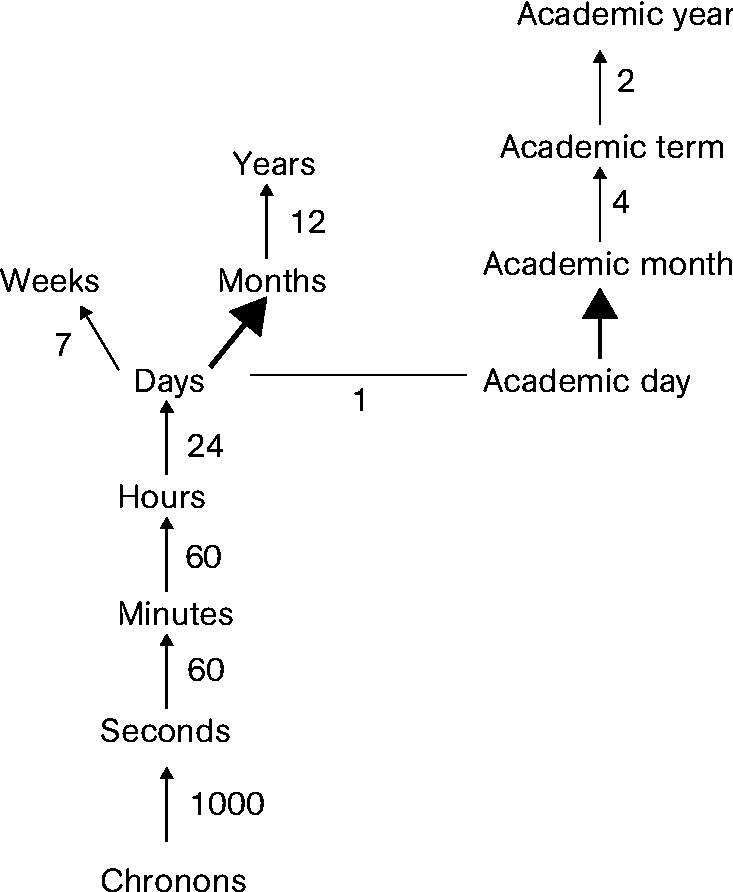
\includegraphics[scale=0.5]{graphs/granularityGraph.pdf}
%\caption{A granularity graph example}
%\label{fig:granularity-graph-example}
%\end{figure}


Next, in subsection \ref{subsec:timedomain-calendar}, some basic concepts and issues concerning calendars are explained.

\subsection{Calendars}
\label{subsec:timedomain-calendar}
%maybe introduce previously the concept of time units, linear hierarchy and time point.

This subsection will concern \emph{calendars}. A calendar provides some sort of human interpretation of time. As such, calendars provide meaning or interpretation to temporal values where this meaning or interpretation is relevant or useful to the user. More precisely, calendars determine the mapping between human-meaningful time values and an underlying time model~\cite{Dyreson1994}. More formally, a calendar is an organization of different granularities (e.g. granularities day, month and year) in a hierarchy. In order to formally define what a calendar is, some other concepts should first be introduced~\cite{Kraus1997}:


%\begin{svgraybox}
%\vspace{-10pt}
%\begin{definition}\textbf{(Calendar)}\\
%A \emph{\textbf{calendar}} 
%\end{definition}
%\vspace{-10pt}
%\end{svgraybox}


\begin{svgraybox}
\vspace{-10pt}
\begin{definition}\textbf{Linear Hierarchy of Granularities}\\
A \emph{\textbf{linear hierarchy of granularities}} is a finite set of granularities with a linear order (denoted $\sqsubset$). The most coarse granularity is called \emph{the top of the hierarchy} and must be an infinite set while all other granularities must be finite sets.
\end{definition}
\vspace{-10pt}
\end{svgraybox}

An example of a linear hierarchy is the set $\left\{ \text{days, months, years} \right\}$, where days $\sqsubset$ months and months $\sqsubset$ years. With this, a \emph{linear calendar} can be defined.

\begin{svgraybox}
\vspace{-10pt}
\begin{definition}\textbf{Linear Calendar}\\
A \emph{\textbf{linear calendar}} consist of a linear hierarchy of granularities and a validity predicate which specifies if a granule is valid in the calendar.
\end{definition}
\vspace{-10pt}
\end{svgraybox}

An example of a linear calendar could be the linear hierarchy $\left\{ \text{days, months, years} \right\}$, where days $\sqsubset$ months and months $\sqsubset$ years, together with a validity predicate that excludes time indications like `32 april 2012' or `30 february 2012'.

%The linear hierarchy days $\sqsubset$ months $\sqsubset$ years represents a linear calendar. It is necessary to define the validity predicates because 17 January 2012 is a valid element of the calendar whereas 30 February 2012 is not.
 
\textcolor{red}{CHECK}
\subsubsection{\label{subsubsubsec:julian-day-number}An example of temporal domain: Julian Day Number}
% proposal for the underlying Julian Day Number domain.

The Julian Day number \emph{JDN} \cite{Dir96} is a counter. Its value is incremented in one unit every day from 1 January 4713 B.C. at 12:00 noon. The particularity of starting at noon was useful for astronomers: the observations they took one night belonged to the same Julian Day.\\
Note that the Julian Day represents whole days. There is an extension that allows to represent any precision needed (it is called Julian Date). By default, a Julian Day is expressed in Universal Time. (U.T, also known as Solar Time). However, there are representations in Terrestrial Time (T.T), Epheris Time (J.E.D. or J.D.E.). Any time scale different from Universal Time must be explicited after the Julian Day number. There are several conversion formulas~\cite{Usn}\cite{Wik}\cite{Lea} between a date in Gregorian calendar  format and a date in  JDN format. The inverse conversion formula is proposed in~\cite{Fliegel:1968:LEM:364096.364097}\\

There are many alternatives to optimize the representation of Julian Day numbers because of its extremely far origin (4713 B.C. year). Table \ref{table:juliandayrepresentations} shows several time domains that can be calculated from the Julian Date, some of them are proposed just for optimization purposes.


\begin{table}
\caption{Julian Day representations}
\label{table:juliandayrepresentations}

\begin{tabular}{p{2cm}p{4cm}p{4cm}p{2cm}}
%header ------------------------------------------------------
\hline\noalign{\smallskip}
Name & From & Formula & Current Value  \\ 
\noalign{\smallskip}\svhline\noalign{\smallskip}
%header ------------------------------------------------------
Julian Date (JD)$^a$ & 12:00 noon Monday 1 January 4713 B.C & & 2455278. 85488  \\ 
Julian Day Number (JDN)$^b$ & 12:00 noon  Monday 1 January 4713 B.C. & JND = floor(JD) & 2455278 \\ 
Reduced Julian Day (RJD)$^c$ & 12:00 noon Tuesday 16 November 1858 A.C. & RJD = JD - 2400000 & 55278.85488  \\ 
Modified Julian Day (MJD)$^d$ & 00:00 Wednesday 17 November 1858 A.C. & MJD = JD - 2400000,5 & 55278.35488 \\ 
Truncated Julian Day (TJD)$^e$ & 00:00 Friday 24 May 1968 A.C. & TJD = JD - 2440000,5 & 15278.35488  \\ 
Truncated Julian Day (TJD)$^f$ & 00:00 Thursday 10 November 1995 A.C. & TJD = (JD- 0,5) mod 10000 & 5278. 35488   \\ 
Dublin Julian Day (DJD))$^g$ & 12:00 noon Sunday 31 December 1899 A.C. & DJD = JD - 2415020 & 40258. 85488 \\ 
Chronological Julian Day (CJD)$^h$  & 00:00 Monday 1 January 4713 B.C. & CJD = JD + 0,5 + timezone adjust. & 2455279. 3548843 (UT)  \\ 
Lilian Day Number$^i$ & Friday 15 October 1582 & floor(JD-2299160,5) & 156118 \\ 
ANSI Date$^j$  & Monday 1 January 1601 & floor(JD-2305812,5) & 149466  \\ 
Rata die$^k$  & Monday 1 January 1 A.C & floor(JD - 1721424.5) & 733854 \\ 
Unix time$^l$  & Thursday 1 January 1970 A.C. & (JD – 2440587.5) × 86400 & 1269333062 \\ 
\noalign{\smallskip}\hline\noalign{\smallskip}
\end{tabular}
$^a$ This is an extension of the Julian Day that allows time representation. \\
$^b$  Each day changes at noon. \\
$^c$  Used by astronomers. \\
$^d$ It starts at midnight. \\
$^e$ Definition from NASA. \cite{Sch}. \\
$^f$ Definition from NIST. \cite{Nis}. \\
$g$ Introduced by the IAU in 1995. \\
$^h$ The timezone must be explicited. Each day changes at midnight. \\
$^i$ The number of days since Gregorian calendar in Universal Time. \\
$^j$ The origin for COBOL integer dates. \\
$^k$  The number of days since actual era. \\
$^l$  It counts the seconds not the day. \\
\end{table}

\textcolor{red}{END CHECK}

The next section briefly introduces temporal relationships.

\subsection{Temporal Relationships}
%an explanation on allen's temporal relations.
%definition of fuzzy temporal interval
In this section, a brief introduction can be found, concerning \emph{temporal relationships}, sometimes also called `temporal relations'\cite{Billiet:Pons:Matthe:DeTre:Pons:2011:BipolarFuzzy}. Temporal relationships can be seen as relationships between temporal elements or instants.

\def\JPicScale{0.5}
\begin{figure}[h]
\centering
%%Created by jPicEdt 1.4.1_03: mixed JPIC-XML/LaTeX format
%%Tue Jan 17 09:05:12 CET 2012
%%Begin JPIC-XML
%<?xml version="1.0" standalone="yes"?>
%<jpic x-min="4" x-max="85" y-min="-2" y-max="140" auto-bounding="true">
%<text text-vert-align= "center-v"
%	 anchor-point= "(4,70)"
%	 fill-style= "none"
%	 text-frame= "noframe"
%	 text-hor-align= "center-h"
%	 >
%I Before J
%</text>
%<multicurve fill-style= "none"
%	 points= "(50,75);(50,75);(80,75);(80,75)"
%	 />
%<multicurve fill-style= "none"
%	 points= "(25,65);(25,65);(45,65);(45,65)"
%	 />
%<text text-vert-align= "center-v"
%	 anchor-point= "(35,67.5)"
%	 fill-style= "none"
%	 text-frame= "noframe"
%	 text-hor-align= "center-h"
%	 >
%I
%</text>
%<text text-vert-align= "center-v"
%	 anchor-point= "(65,77.5)"
%	 fill-style= "none"
%	 text-frame= "noframe"
%	 text-hor-align= "center-h"
%	 >
%J
%</text>
%<text text-vert-align= "center-v"
%	 anchor-point= "(4,56)"
%	 fill-style= "none"
%	 text-frame= "noframe"
%	 text-hor-align= "center-h"
%	 >
%I Equal J
%</text>
%<text text-vert-align= "center-v"
%	 anchor-point= "(20,140)"
%	 fill-style= "none"
%	 text-frame= "noframe"
%	 text-hor-align= "center-h"
%	 >
%
%</text>
%<multicurve fill-style= "none"
%	 points= "(20,85);(20,85);(20,0);(20,0)"
%	 />
%<multicurve right-arrow= "head"
%	 fill-style= "none"
%	 points= "(20,0);(20,0);(85,0);(85,0)"
%	 />
%<text text-vert-align= "center-v"
%	 anchor-point= "(80,-2)"
%	 fill-style= "none"
%	 text-frame= "noframe"
%	 text-hor-align= "center-h"
%	 >
%Time
%</text>
%<multicurve fill-style= "none"
%	 points= "(25,55);(25,55);(45,55);(45,55)"
%	 />
%<text text-vert-align= "center-v"
%	 anchor-point= "(35,57.5)"
%	 fill-style= "none"
%	 text-frame= "noframe"
%	 text-hor-align= "center-h"
%	 >
%J
%</text>
%<text text-vert-align= "center-v"
%	 anchor-point= "(4,46)"
%	 fill-style= "none"
%	 text-frame= "noframe"
%	 text-hor-align= "center-h"
%	 >
%I Meets J
%</text>
%<text text-vert-align= "center-v"
%	 anchor-point= "(40,40)"
%	 fill-style= "none"
%	 text-frame= "noframe"
%	 text-hor-align= "center-h"
%	 >
%
%</text>
%<multicurve fill-style= "none"
%	 points= "(45,45);(45,45);(65,45);(65,45)"
%	 />
%<text text-vert-align= "center-v"
%	 anchor-point= "(55,47.5)"
%	 fill-style= "none"
%	 text-frame= "noframe"
%	 text-hor-align= "center-h"
%	 >
%J
%</text>
%<text text-vert-align= "center-v"
%	 anchor-point= "(6,36)"
%	 fill-style= "none"
%	 text-frame= "noframe"
%	 text-hor-align= "center-h"
%	 >
%I Overlaps J
%</text>
%<multicurve fill-style= "none"
%	 points= "(30,35);(30,35);(50,35);(50,35)"
%	 />
%<text text-vert-align= "center-v"
%	 anchor-point= "(40,37.5)"
%	 fill-style= "none"
%	 text-frame= "noframe"
%	 text-hor-align= "center-h"
%	 >
%J
%</text>
%<text text-vert-align= "center-v"
%	 anchor-point= "(4,26)"
%	 fill-style= "none"
%	 text-frame= "noframe"
%	 text-hor-align= "center-h"
%	 >
%I During J
%</text>
%<multicurve fill-style= "none"
%	 points= "(20,25);(20,25);(50,25);(50,25)"
%	 />
%<text text-vert-align= "center-v"
%	 anchor-point= "(35,27.5)"
%	 fill-style= "none"
%	 text-frame= "noframe"
%	 text-hor-align= "center-h"
%	 >
%J
%</text>
%<text text-vert-align= "center-v"
%	 anchor-point= "(4,16)"
%	 fill-style= "none"
%	 text-frame= "noframe"
%	 text-hor-align= "center-h"
%	 >
%I Starts J
%</text>
%<multicurve fill-style= "none"
%	 points= "(25,15);(25,15);(55,15);(55,15)"
%	 />
%<text text-vert-align= "center-v"
%	 anchor-point= "(6,6)"
%	 fill-style= "none"
%	 text-frame= "noframe"
%	 text-hor-align= "center-h"
%	 >
%I Finishes J
%</text>
%<text text-vert-align= "center-v"
%	 anchor-point= "(35,17.5)"
%	 fill-style= "none"
%	 text-frame= "noframe"
%	 text-hor-align= "center-h"
%	 >
%J
%</text>
%<text text-vert-align= "center-v"
%	 anchor-point= "(35,7.5)"
%	 fill-style= "none"
%	 text-frame= "noframe"
%	 text-hor-align= "center-h"
%	 >
%J
%</text>
%<multicurve fill-style= "none"
%	 points= "(25,5);(25,5);(45,5);(45,5)"
%	 />
%<text text-vert-align= "center-v"
%	 anchor-point= "(6,80)"
%	 fill-style= "none"
%	 text-frame= "noframe"
%	 text-hor-align= "center-h"
%	 >
%Relations
%</text>
%</jpic>
%%End JPIC-XML
%LaTeX-picture environment using emulated lines and arcs
%You can rescale the whole picture (to 80% for instance) by using the command \def\JPicScale{0.8}
\ifx\JPicScale\undefined\def\JPicScale{1}\fi
\unitlength \JPicScale mm
\begin{picture}(85,140)(0,0)
\put(4,70){\makebox(0,0)[cc]{I Before J}}

\linethickness{0.3mm}
\put(50,75){\line(1,0){30}}
\linethickness{0.3mm}
\put(25,65){\line(1,0){20}}
\put(35,67.5){\makebox(0,0)[cc]{I}}

\put(65,77.5){\makebox(0,0)[cc]{J}}

\put(4,56){\makebox(0,0)[cc]{I Equal J}}

\put(20,140){\makebox(0,0)[cc]{}}

\linethickness{0.3mm}
\put(20,0){\line(0,1){85}}
\linethickness{0.3mm}
\put(20,0){\line(1,0){65}}
\put(85,0){\vector(1,0){0.12}}
\put(80,-2){\makebox(0,0)[cc]{Time}}

\linethickness{0.3mm}
\put(25,55){\line(1,0){20}}
\put(35,57.5){\makebox(0,0)[cc]{J}}

\put(4,46){\makebox(0,0)[cc]{I Meets J}}

\put(40,40){\makebox(0,0)[cc]{}}

\linethickness{0.3mm}
\put(45,45){\line(1,0){20}}
\put(55,47.5){\makebox(0,0)[cc]{J}}

\put(6,36){\makebox(0,0)[cc]{I Overlaps J}}

\linethickness{0.3mm}
\put(30,35){\line(1,0){20}}
\put(40,37.5){\makebox(0,0)[cc]{J}}

\put(4,26){\makebox(0,0)[cc]{I During J}}

\linethickness{0.3mm}
\put(20,25){\line(1,0){30}}
\put(35,27.5){\makebox(0,0)[cc]{J}}

\put(4,16){\makebox(0,0)[cc]{I Starts J}}

\linethickness{0.3mm}
\put(25,15){\line(1,0){30}}
\put(6,6){\makebox(0,0)[cc]{I Finishes J}}

\put(35,17.5){\makebox(0,0)[cc]{J}}

\put(35,7.5){\makebox(0,0)[cc]{J}}

\linethickness{0.3mm}
\put(25,5){\line(1,0){20}}
\put(6,80){\makebox(0,0)[cc]{Relations}}

\end{picture}

\caption{Allen relations between two time intervals.}
\label{fig:allen}
\end{figure}

Several operators are defined in order to compare temporal elements or time points. Allen~\cite{Allen83} first described the relationships between time intervals and as a special case, between time points. Figure \ref{fig:allen} shows the temporal relationships Allen discerned. Some proposals can be applied to both crisp and fuzzy temporal intervals~\cite{ohlbach2004},~\cite{nagypal2003},~\cite{schockaert08}. 

\textcolor{red}{MOVE TO FUZZY PART}
For this fuzzy comparisons~\cite{garrido2009} proposed some different temporal relations that can be easily implemented by means of regular fuzzy operations.
\textcolor{red}{END MOVE TO FUZZY PART}

In the next section, some basic concepts and terminology about temporal databases are presented, followed by an overview of some interesting issues concerning temporal databases and a survey of some commercial temporal database systems.